\documentclass[12pt]{article}

\usepackage{amsmath}
\usepackage[authoryear,round]{natbib}
%\usepackage{hyperref}




\textwidth=6.2in
\textheight=8.5in
\oddsidemargin=.1in
\evensidemargin=.1in
\headheight=-.3in

\newcommand{\scscst}{\scriptscriptstyle}
\newcommand{\scst}{\scriptstyle}
\newcommand{\Rfunction}[1]{{\texttt{#1()}}}
\newcommand{\Rmethod}[1]{{\texttt{#1}}}  
\newcommand{\Rclass}[1]{{\texttt{#1}}}
\newcommand{\Robject}[1]{{\texttt{#1}}}
\newcommand{\Rpackage}[1]{{\textit{#1}}}
\newcommand{\code}[1]{{\texttt{#1}}}
\bibliographystyle{plainnat}
\def\tm{$^{\rm \text{TM }}$}

\title{Analysis of High Throughput Flow Cytometry Data using \Rpackage{plateCore}}

%%%%%%%%%%%%%%%%%%%%%%%%%%%%%%%%%%%%%%%%%%%%%%%%%%%%%%%%%%%%%%%%%%%%%%%%%%%
\usepackage{Sweave}
\begin{document}
\maketitle

\clearpage
%%%%%%%%%%%%%%%%%%%%%%%%%%%%%%%%%%%%%%%%%%%%%%%%%%%%%%%%%%%%%%%%%%%%%%%%%%%%%%%%%%%%%%%%%%%%%%%%%%%%%%%%%%%%%%%%%%%%%%%%%%%%%%%%%%%
\section*{Abstract}
\subsection*{Background}
High throughput flow cytometry (FCM) studies are often run in a 96 or 384-well plate format, with a number of different samples, 
controls, and antibodies-dye conjugates present on each plate. 
Analyzing a plate requires tracking the contents
of each well, matching sample wells with control wells, gating each well/channel separately, making the appropriate plots,
assessing quality, and finally aggregating the results from multiple plates into an experiment level data object. 
This analysis can be a monumental task using traditional point-and-click software packages, even when multiple instances are
deployed. We developed \Rpackage{plateCore} as an R/Bioconductor packaged to make processing and analysis of
large, complex datasets easier. 

\subsection*{Methods}
\Rpackage{plateCore} was used to analyze the data from a BD FACS\tm CAP screening experiment where 5
Peripheral Blood Mononucleocyte Cell (PBMC) samples 
were assayed for 189 different human cell surface markers. 
This same dataset was also analyzed by a cytometry expert using FlowJo\tm.

\subsection*{Results}
Positive markers identified using \Rpackage{plateCore} are in good agreement with those found using FlowJo\tm analysis.

\subsection*{Conclusions}
\Rpackage{plateCore} provides a reproducible, objective platform for analyzing high throughput flow experiments. The R/Bioconductor 
implementation allows bioinformaticians and statisticians access to the data, which should further the development of automated
analysis methods.

\clearpage
%%%%%%%%%%%%%%%%%%%%%%%%%%%%%%%%%%%%%%%%%%%%%%%%%%%%%%%%%%%%%%%%%%%%%%%%%%%%%%%%%%%%%%%%%%%%%%%%%%%%%%%%%%%%%%%%%%%%%%%%%%%%%%%%%%
\section*{Introduction}

While there are a number of different software packages available for analysis of flow cytometry data, these programs are often
ill-suited to the development of new methods needed for analyzing high-throughput flow studies.
Flow Cytometry High Content Screening (FC-HCS) experiments generate large volumes of data, and a systematic approach to
preprocessing, gating (i.e. filtering), and summarizing results is needed for robust analyses. 
Ideally these steps would be automated,
allowing analysis pipelines to be robust, objective, and match the high-throughput capacity of modern cytometers. 
Unfortunately, current approaches to FC-HCS analysis are semi-automated at best,
and they often significant manual intervention to identify cells of interest and set the appropriate gates. 
Since the manual contribution is subjective and prone to error when working with large numbers of samples \citep{Maecker2005},
it is desirable to develop programmatic approaches to process the data.

Flow cytometry packages available through the Bioconductor \citep{BIOC} project provide an open platform that
can be used by cytometrists, bioinformaticians, and statisticians to collaboratively develop new methods for
automated FC-HCS analysis.  The basic data processing tools for importing, transforming, gating, and
organizing raw flow cytometry data are in the \Rpackage{flowCore} package \citep{hahne2009}, and the visualization functions are
in \Rpackage{flowViz} \citep{sarkar2008ufv}. The Bioconductor model for flow data analysis facilitates
the development of new analysis methods, since the overhead associated with
accessing and visualizing flow data is handled by \Rpackage{flowCore} and \Rpackage{flowViz}.
The availability of \Rpackage{flowCore} and \Rpackage{flowViz} has enabled the creation of new tools for
quality assessment of large flow experiments, such as \Rpackage{flowQ} \citep{lemeurFQ}, and model-based clustering and automated
gating, such as \Rpackage{flowClust} \citep{lo2008}.
\Rpackage{plateCore} also takes advantage of the functionality in \Rpackage{flowCore} and \Rpackage{flowViz}
to create methods and data structures for processing large, plate-based flow datasets.  

An example of the progression from raw FCM data files to a completed \Rpackage{plateCore} analysis is shown in Figure~\ref{fig:analysis}.
List mode FCS files for a single plate are read into a \Robject{flowSet} using \Rpackage{flowCore}, and then a \Robject{flowPlate} is created by integrating
the plate annotation file with the \Robject{flowSet}. The \Robject{flowPlate} is then compensated, data quality is assessed, and gates
are set according to a negative control. These control gates are then applied to test wells to find cells that have specific staining
in channels of interest. While this same analysis can be performed relatively quickly in 
other flow cytometry software packages, it can be difficult to reproduce the gating decisions made by a single expert user.

In addition to subjective gating, the lack of a standard format for describing large flow experiments also
makes it difficult for anyone other than the original experimenter to replicate an analysis. 
The adoption of ACS specifications (http://www.ficcs.org/data-standards.html) should make it easier to access metadata in future flow studies, but currently
this information is typically provided either as spreadsheet or a pictorial layout of a 96 well plate. 
Since the creation of \Robject{flowPlate} requires users to make a standard sample annotation file, plate layouts from \Rpackage{plateCore}
can then be easily shared along with the raw FCS2.0/3.0 files. 
The standard format for \Rpackage{plateCore} sample annotations provides a convenient way to manage the plate metadata
associated with complex FC-HCS experiments.

\Rpackage{plateCore} is not designed to be a GUI driven end-user tool, but rather to help develop a standardized platform for the analysis of FC-HCS data.
These analyses often represent a collaborative effort between cytometry experts who generate the data and the quantitative individuals who help
deal with the large volume information. In order for this collaboration to work, the cytometrists must have confidence in the
results of the automated analysis. To this point, we demonstrate the equality of our results to those produced by an expert
cytometrist using FlowJo\tm.


\begin{figure}
\centering
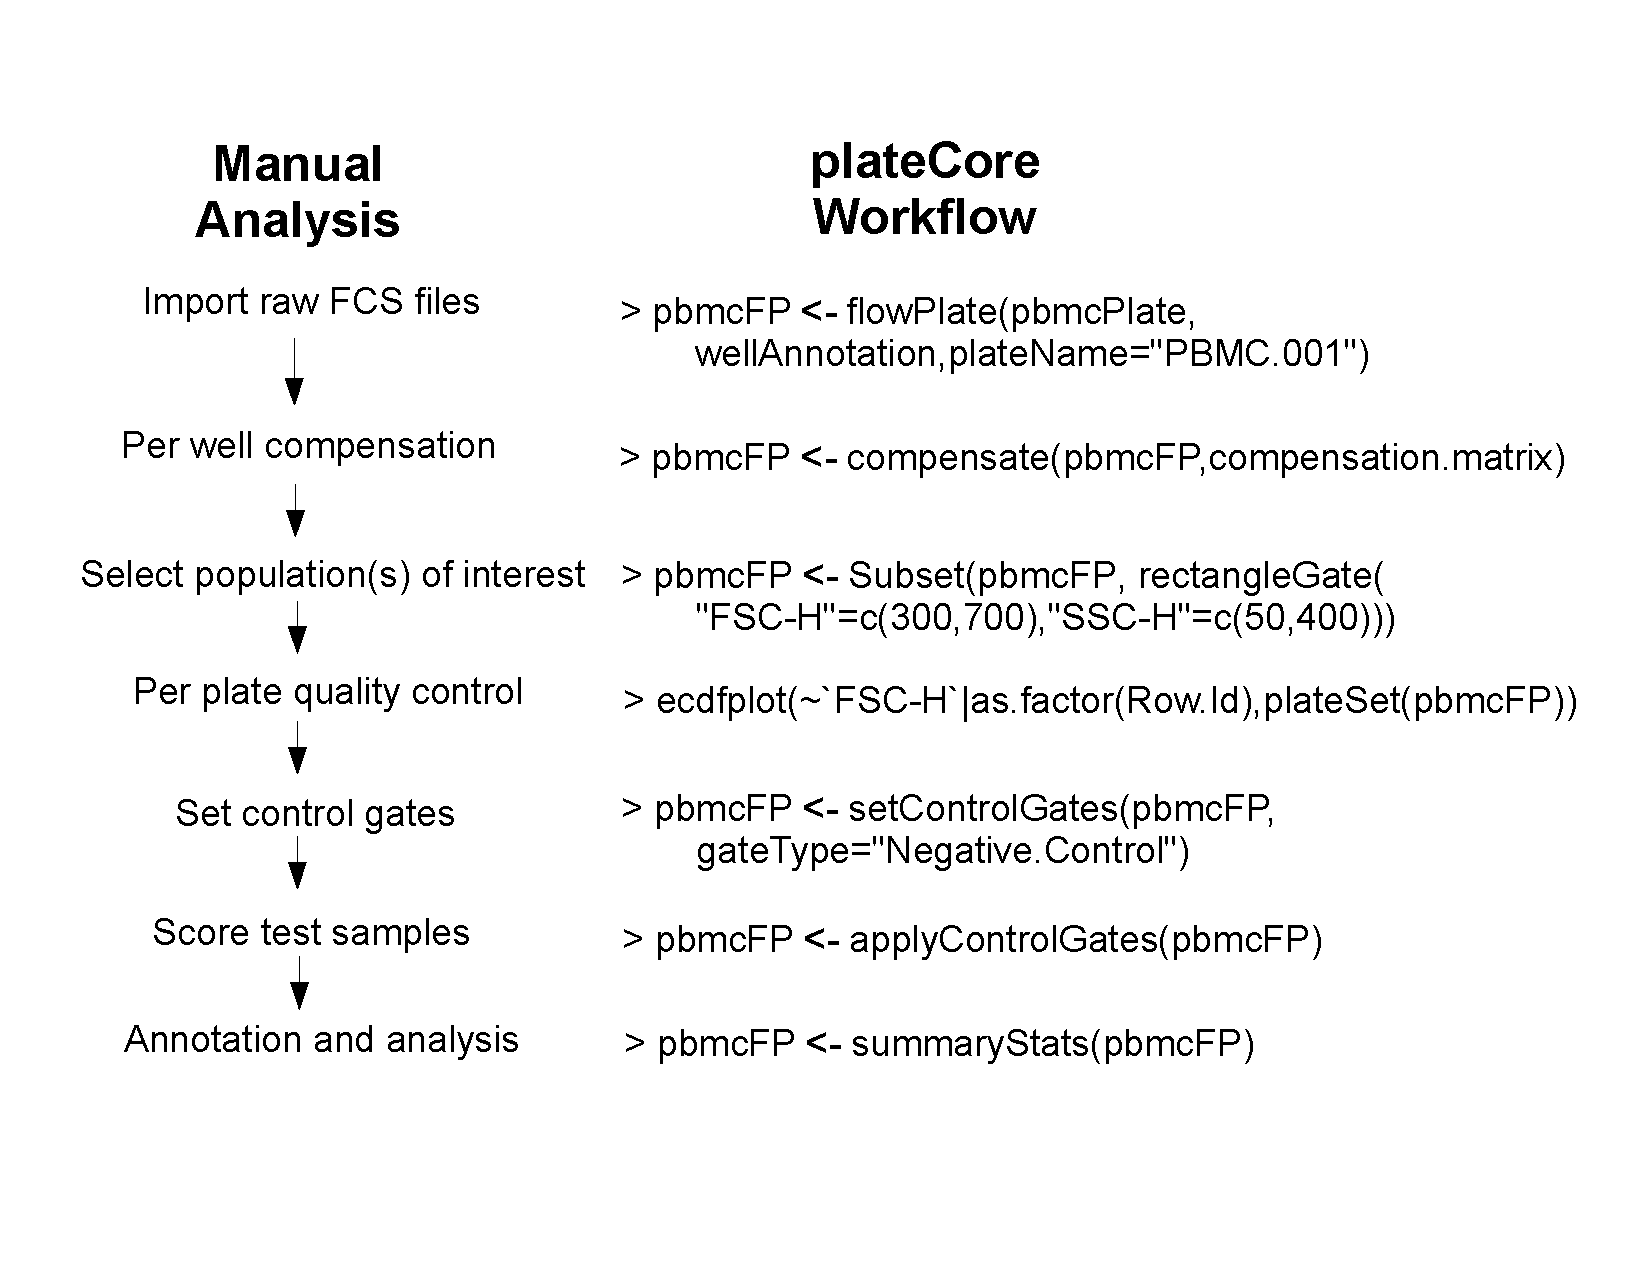
\includegraphics[width=7in,height=6in]{analysisSteps.pdf}
\caption{Typical FC-HCS plate workflow on the left and corresponding steps from a PBMC lymphocyte plateCore analysis on the right.
Compared to analyses performed using existing GUI FCM tools, plateCore can reduce the level of subjectivity associated with creating
the negative control gates and also makes it easier to aggregate multiple plates into an experiment level object for visualization and reporting.
Providing plateCore scripts along with the raw FCM data for FC-HCS experiments helps to ensure that the analysis is transparent and reproducible.
}
\label{fig:analysis}
\end{figure}
 
%%%%%%%%%%%%%%%%%%%%%%%%%%%%%%%%%%%%%%%%%%%%%%%%%%%%%%%%%%%%%%%%%%%%%%%%%%%%%%%%%%%%%%%%%%%%%%%%%%%%%%%%%%%%%%%%%%%%%%%%%%%%%%%%%%%
\clearpage
\section*{Materials and Methods}
\subsection*{Data}

BD FACS\tm CAP was designed as a cell characterization tool to screen for the presence a large number of different human 
cell surface markers. In this study, PBMC samples (previously frozen) from two donors were analyzed on a BD FACScalibur
using BD FACS\tm CAP staining. The analysis was performed on 96-well plates with
189 different antibodies arrayed 3 per well in 63 test wells, along with 30 isotype control wells and 3 unstained controls.
The complete list of BD FACS\tm CAP antibodies can be found at http://www.bd.com/technologies/discovery\_platform/BD\_FACS\_CAP.asp. 
FCM files for the 5 plates, 2 for donor 1 and 3 for donor 2, are available for download from http://www.ficcs.org.

%%%%%%%%%%%%%%%%%%%%%%%%%%%%%%%%%%%%%%%%%%%%%%%%%%%%%%%%%%%%%%%%%%%%%%%%%%%%%%%%%%%%%%%%%%%%%%%%%%%%%%%%%%%%%%%%%%%%%%%%%%%%%%%%%%%
\subsection*{Analysis}

The goal of the PBMC FACS\tm CAP study was to look for positive staining for the 189 different cell
surface markers in lymphocytes. The \Rpackage{plateCore} scripts used to perform the analysis are provided 
in supplementary materials. Briefly, the FCM files are first processed using a combination of static (\Robject{rectangleGate})
and data driven (\Robject{norm2filter}) \Rpackage{flowCore} gates to pick out the lymphocytes in the forward (FSC) and side scatter (SSC)
channels.  The quality of the data was then assessed by looking for fluidic events such as bubbles,
pressure drops, or large aggregates that can shift the baseline fluorescence readings. 
Fluidic events can often be identified by plotting the emprical cumulative density (ecdf) plots of FSC
values for each well, and looking for distributions shifted relative to other wells \citep{lemeur2007}. Based on the ecdf
plots, several wells were further investigated by cytometry experts who determined that the shifts were in an acceptable range.
Next the threshold between positive and negative cells are determined using the isoytpe controls, which provide a gross estimate
of non-specific binding in the primary antibodies. One-dimensional gates are created using using the isotype thresholds, and these
gates are applied to identify cells that are positively stained for each marker. 

In addition to \Rpackage{plateCore}, the 5 PBMC plates were also analyzed using FlowJo$^{\text{TM}}$,
which is one of the standard FCM data analysis platforms. First, an analysis template is created
where test wells and their corresponding isotype control well are assigned to one of 30 groups. Wells in each
group have similar sets of antibody-dye conjugates, and the expression threshold (i.e. isotype gate)
is initially set using the isotype control well. Data for each plate was imported into FlowJo$^{\text{TM}}$
using the template and
lymphocytes were selected using a morphology (FSC-SSC) gate. Event data for the isotype well was then
visualized on a log scale, and the expression threshold for each stained channel was set by picking a
value that lies above the bulk of the events. For BD FACS\tm CAP, the isotype gate is set so that less than
1\% of the events in the isotype well are above the threshold. These gates are then applied to the test
wells, and the threshold may be moved up or down based on positive test wells. The percentage
of cells above the threshold for each of the 189 antibodies is then exported to a separate spreadsheet for 
each plate.

%%%%%%%%%%%%%%%%%%%%%%%%%%%%%%%%%%%%%%%%%%%%%%%%%%%%%%%%%%%%%%%%%%%%%%%%%%%%%%%%%%%%%%%%%%%%%%%%%%%%%%%%%%%%%%%%%%%%%%%%%%%%%
\section*{Results}

\subsection*{\Rpackage{plateCore}}
The 5 PBMC plates were analyzed using the approach shown in Figure~\ref{fig:analysis}.  Results
are stored in \Robject{flowPlates}, which are data structures that contain a description of the
plate layout, morphology gated (FSC-SSC) events, and parameters values for the 
the negative control gates (i.e. isotype gates). Event level data can be 
visualized using plotting functions from \Rpackage{plateCore} and \Rpackage{flowViz}. 
Additionally, results from different plates can be aggregated, making it easier to compare
results from different plates and to create the complex reports required to summarize results from 
189 different markers.

One hundred and nine of the 189 markers were positive on at least one plate.
Positive for BD FACS\tm CAP was defined as having more than 10\% of
events above the isotype gate. Since antibody concentrations used in BD FACS\tm CAP are designed
to screen a number of different cell types, the concentrations are not necessarily optimal for these PBMC samples. 
The 10\% cutoff is an empirically determined threshold (data not shown) used to select markers for further analysis,
including single color titration and competition experiments to confirm that the marker is present
and staining is specific. Markers that are highly positive ($\ge$ 90\%) are usually confirmed in
follow-up studies, while markers that are low positives ($\le$ 15\%) are often the result of non-specific
staining. Also, these percentages refer to the fraction of events above the isotype threshold, but
this does not necessarily imply heterogeneous staining in multiple populations.

Since the majority of antibodies on the BD FACS\tm CAP staining plate are known to bind different
leukocytes, it is not surprising that a large fraction would be identified as positive on PBMCs.  Markers such
as CD44, CD45, CD47, and CD59 are broadly expressed on lymphocytes and show show up as highly positive (>99\%)
in this study. Markers that are expressed on a small subset of lymphocytes, or markers that are dimly expressed,
would not be found with this screening approach. The difficulty in determining whether a dim marker
is expressed can be seen in Figure~\ref{fig:mfiRatio}, where samples with Median Fluorescence Intensity (MFI)
ratios between 1 and 10 ranged from 0 to 100\% percent positive.
If the isotype gate is near the MFI of the test well
signal, then estimates of the percentage of positive cells will be unstable.




\clearpage
\begin{figure}
\centering
\includegraphics{outline-mfiRatio}
\caption{Plot of the Median Fluorescence Intensity (MFI) ratio for each of the 189 antibody-dye conjugates
versus the percentage of positive cells identified using plateCore from the 5 PBMC plates.
The MFI ratio refers to the ratio of the test well MFI to the corresponding isotype control on a linear scale.
Cell populations with MFIs that are close to the isotype control are often split by the isotype
gate, reflecting the range of percent positive values for MFI ratios between 1 and 10.}
\label{fig:mfiRatio}
\end{figure}

\clearpage
\subsection*{Comparison to FlowJo\tm Results}
Automating the creation and modification of isotype gates made by cytometrists analyzing BD FACS\tm CAP data
using FlowJo\tm is extremely challenging. Cytometrists adjust gates based on expert knowledge about the performance of 
specific antibody types and dyes, or after identifying positive test samples. The automated approach
employed in \Rpackage{plateCore} determines the threshold using isotype controls.  The gate (G$_{ij}$) for isotype $i$, channel $j$
is set according to:
\begin{equation}
\text{G}_{ij} = \max (\text{99th}_{ij} \text{, MFI}_{ij}+ 4 \text{MAD}_{ij}),
\label{isoGate}
\end{equation}
where 99th$_{ij}$ is the 99th percentile for the fluorescence signal,
MFI is the Median Fluorescence Intensity, and MAD is Median Absolute Deviation
on a linear scale. While this simple, non-parametric method works surprisingly well for BD FACS\tm CAP,
advances in model-based clustering methods, such as those in \Rpackage{flowClust}, should lead
to future performance improvements in automated gating. Comparisons of the \Rpackage{plateCore} and FlowJo\tm 
analysis are shown in Figure~\ref{fig:pcVSman}.

Looking in detail at one case where the \Rpackage{plateCore} and FlowJo\tm methods disagree, such
as CD98 on plate 9208 (Figure~\ref{fig:disagree}), highlights situations where our automated gating
approach will fail. In this case the marker is positive (86\% by FlowJo\tm) but is 
called negative (0\%) by \Rpackage{plateCore}. The isotype control (well H08 in Figure~\ref{fig:disagree})
has >1\% of its events in the FL1-H channel that are above the main population, resulting in the automated
gate being set at the 99th percentile instead of the MFI+4MADS. Fortunately, this type of mistake can also
be detected by looking the MFI ratio plot in Figure~\ref{fig:mfiRatio}. CD98 for plate 9208 has an MFI
ratio of 5 and a percent positive value of 0\%, while other markers with a similar MFI ratio have values
near 70\%. Percent positive values that lie far from the sigmoid curve in Figure~\ref{fig:mfiRatio}
should be evaluated manually.

%Setting the isotype gate using the our approach still requires subjective decisions regarding the 
%fluorescence percentile and number of MADS, but these values have shown little variation within the different cell types
%that have been assayed using BD FACS\tm CAP (results not shown). Within a particular cell type we 
%are able to replicate the gating decisions made by cytometrists. If we encounter a new cell type or if the analysis
%is performed using a different cytometer, then the gate settings must be reevaluated. 

\clearpage
\begin{figure}
\centering
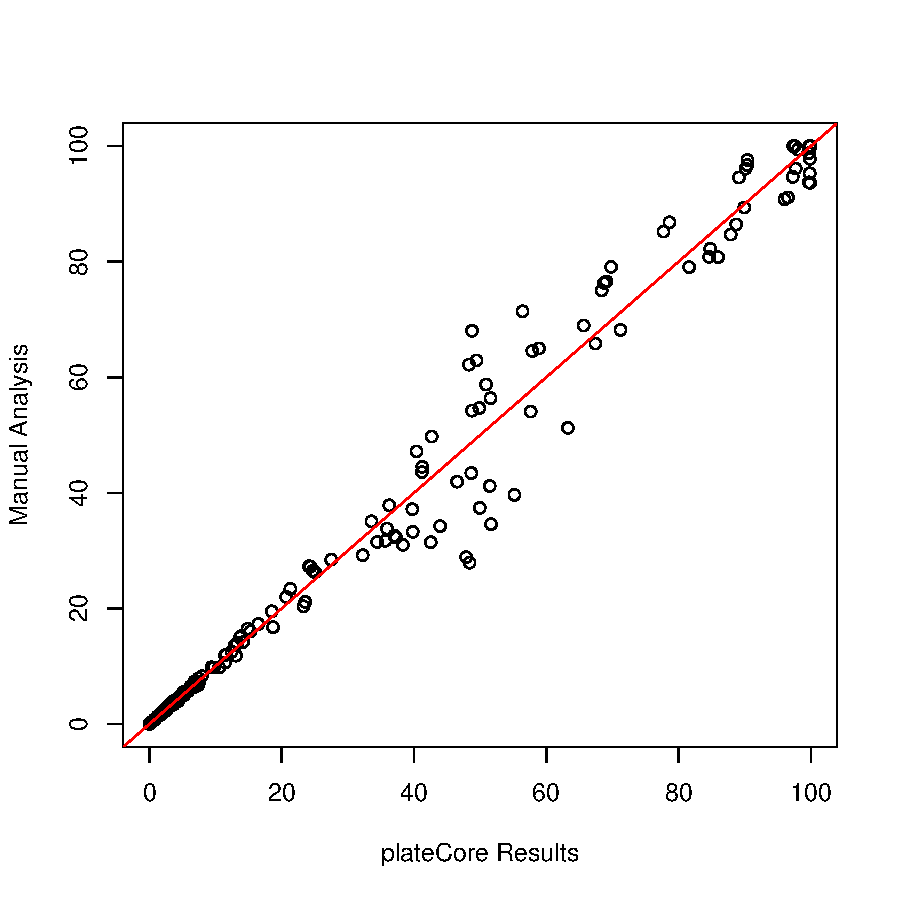
\includegraphics{outline-pcVSman}
\caption{Percent positive results for 189 BD FACS\tm CAP markers analyzed using either \Rpackage{plateCore}
or FlowJo\tm for the 5 PBMC plates. Markers that varied the most between the the two methods tended to have
intermediate percent positive values (30\% to 70\%), reflecting the difficulty of gating populations whose MFI is 
near the isotype threshold. Additionally, since BD FACS\tm CAP was designed as screening tool to 
identify markers for further analysis, false negatives are a bigger concern than false positives. The plateCore
settings were chosen to err on the side of calling samples positive.
}
\label{fig:pcVSman}
\end{figure}

\clearpage
\begin{figure}
\centering
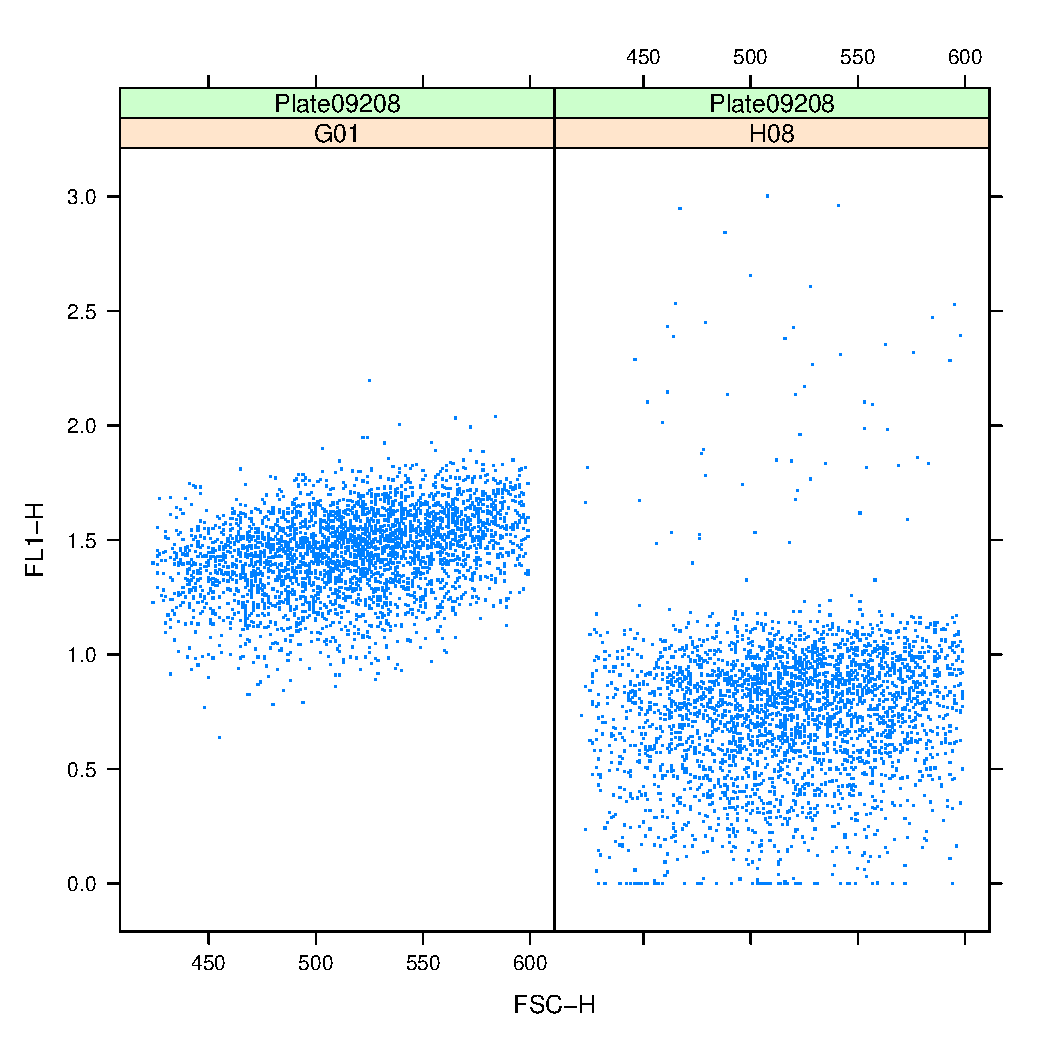
\includegraphics{fjVSr2.pdf}
\caption{Dotplot for CD98 in well G01 and its isotype control well H08 for plate 9208. FlowJo\tm
(86\%) and plateCore (0\%) reported dramatically different percent positive values for this marker. The 
difference was caused by the isotype well having >1\% of the events above the main population, which
resulted in the automated gate being set at the 99th\% instead of the MFI+4MADs.}
\label{fig:disagree}
\end{figure}


%%%%%%%%%%%%%%%%%%%%%%%%%%%%%%%%%%%%%%%%%%%%%%%%%%%%%%%%%%%%%%%%%%%%%%%%%%%%%%%%%%%%%%%%%%%%%%%%%%%%%%%
\clearpage
\subsection*{Donor Variation}

A common goal for BD FACS\tm CAP screens is to identify markers that show variation in expression levels
among cells isolated from different donors. Variation in estimates of the percentage of positive cells can
be modeled using a binomial, where markers that are clearly positive or negative (0 or 100\%) have little
variation and those near the isotype gate (50\%) are highly variable.
Unfortunately, the power to detect differences in this study is limited
since there are only 2 donors and the level of replication is low (2-3 plates per donor).
Figure~\ref{fig:donorVar} shows  the expected and observed variation in the percentage of
positively stained cells for the 189 markers. Discounting CD98, which had an unusual isotype control, the
markers with the most variation (S.D. near 30\%) were CD85, CD97, CD154, CD184, and CD252. Since CD85, CD97, CD154, and 
CD252 are associated with activated T-cells, it is tempting to speculate that this difference represents
biological variation between the two donors as opposed to technical differences in the processing and gating
of the cells.

\begin{figure}
\centering
\includegraphics{outline-donorVar}
\caption{Scatterplot showing the mean percentage of positive cells for each positive marker
versus the observed (circles) and expected (line) sample standard deviation. Expected
values follow a binomial distribution with n=5. Markers that lie above the expected line will be 
further evaluated using titration and competition experiments to see if these results represent
real variation between the two donors. The curve in the expected line reflects the difficulty
in gating samples whose median signal (MFI) is near the isotype cutoff, since the percentage of positive 
cells calculated can shift dramatically with small changes in the gate.}
\label{fig:donorVar}
\end{figure}

%\begin{figure}
%\centering
%<<label=pbmcCDbd69,fig=TRUE,echo=FALSE>>=
%
%fileNames <- list.files("../../publicationPlateCore/pbmcRData",full.names=TRUE)
%
%plates <- lapply(fileNames,function(x){
%			load(x)
%			platePBMC[c("A03","B06")]
%		})
%
%virtPlate <- fpbind(plates[[1]],plates[[2]],plates[[3]],plates[[4]],plates[[5]])
%
%
%print(densityplot(~ `FL2-H` | as.factor(plateName), transform("FL2-H"=log10) %on% virtPlate,
%				filterResult="Negative.Control",col=c('red','blue')))
%
%@
%\caption{Histograms for CDbd69, which is one of the 3 candidates for differential expression from Figure~\ref{fig:donorVar}.
%Isotypes are shown in red and test wells are in blue. Similar plots were automatically created using \Rpackage{plateCore}
%for each of 189 markers assayed in this experiment, allowing cytometry experts to quickly survey the results from the 5
%different plates.}
%\label{fig:pbmcCDbd69}
%\end{figure}


%%%%%%%%%%%%%%%%%%%%%%%%%%%%%%%%%%%%%%%%%%%%%%%%%%%%%%%%%%%%%%%%%%%%%%%%%%%%%%%%%%%%%%%%%%%%%%%%%%%%%%%%%%%%%%%%%%%%%%%%%%%%%%%%%%%
\clearpage
\section*{Discussion}

Our approach to this PBMC BD FACS\tm CAP study relied on processing the raw data
in parallel using both FlowJo\tm and \Rpackage{plateCore}. FlowJo\tm
allowed the ctyometrists to thoroughly investigate individual wells, and gave them confidence
that the \Rpackage{plateCore} results were correct (see Figure~\ref{fig:pcVSman}). Using
\Rpackage{plateCore}, we were able to reduce the level subjectivity in setting isotype gates,
eliminate mistakes associated with manual export and merging of plate output,
and automate the creation of plots and data quality reports that summarized the experiment. 
Additionally, the \Rpackage{plateCore} scripts and experimental annotation can
be shared with other cytometry groups, allowing them to reproduce our analysis. 

The complexity of large flow experiments, like BD FACS\tm CAP, highlight the 
difficulty of applying existing flow analysis platforms to high-throughput studies. Generating and
interpreting results from this PBMC study required extensive collaboration between flow cytometrists,
bioinformaticians, and statisticians. At various points in the analysis, each group needed to access
the raw data, annotation, and details about the experimental design. Providing this access using
stand-alone flow platforms is expensive in terms of the price of multiple software licenses
and in time spent training statisticians and bioinformaticians to use the programs. 
Fortunately the Bioconductor flow packages are modeled on standard data structures used for 
microarrays, which should already be familiar to most quantitative individuals working on 
high-throughput biological problems. We found that \Rpackage{flowCore}, \Rpackage{flowViz},
and \Rpackage{plateCore} provided an open analysis platform that facilitated communication between
the flow cytometrists generating the data, and the computational experts analyzing the data.


%%%%%%%%%%%%%%%%%%%%%%%%%%%%%%%%%%%%%%%%%%%%%%%%%%%%%%%%%%%%%%%%%%%%%%%%%%%%%%%%%%%%%%%%%%%%%%%%%%%%%%%%%%%%%%%%%%%%%%%%%%%%%%%%%%%
\clearpage
\bibliographystyle{plain}
\bibliography{outline} 

\end{document}
